\documentclass[tikz,border=2mm]{standalone}
\usetikzlibrary{arrows}

\tikzstyle{arrow} = [->,>=stealth]

\begin{document}

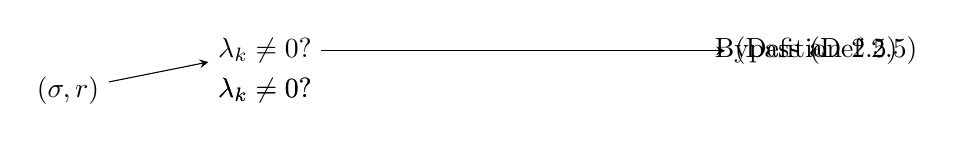
\begin{tikzpicture}[node distance=2cm]

% Nodes
\node (start) {$(\sigma, r)$};
\node (decision1) [right of=start, xshift=0.5cm, yshift=0.5cm] {$\lambda_k \neq 0$?};
\node (bypass1) [right of=decision1, xshift=5cm] {(Defition 2.5)};
\node (decision2) [right of=start, xshift=0.5cm] {$\lambda_k = 0$?};
\node (bypass2) [right of=decision1, xshift=5cm] {Bypass (Def 2.5)};
\node (decision3) [right of=start, xshift=0.5cm] {$\lambda_k \neq 0$?};
\node (bypass3) [right of=decision1, xshift=5cm] {a};
% Arrows
\draw [arrow] (start) -- (decision1);
\draw [arrow] (decision1.east) -- ++(1,0) |- (bypass1.west);

\end{tikzpicture}

\end{document}